%% -*- latex -*-
\documentclass[a4paper]{tufte-handout}

\usepackage[british]{babel}
\usepackage{booktabs}
\usepackage{tikz}
\usepackage{tikz-timing}
\usepackage{minted}
\usepackage{graphicx}
\usepackage{natbib}
\usepackage{siunitx}
\usepackage[theorems,skins]{tcolorbox}
\tcbset{enhanced}
\newtcbtheorem{exercise}{Exercise}{drop fuzzy shadow}{ex}
\newtcbtheorem{question}{Question}{drop fuzzy shadow}{q}

\title{LPC4088 LED Device Driver\\\small{CM0506 Small Embedded Systems}}
\author{Dr Alun Moon}
\date{Seminar 5a}
\definecolor{code}{wave}{602}
%\definecolor{cmd}{wave}{528}
\definecolor{cmd}{named}{SkyBlue}

\begin{document}
\maketitle
\section{LED Driver}
Without an operating system, there is not the need for the complexity
of a Hardware Abstraction Layer.  It can be argued that since the the
hardware of the embedded system is fixed at design time, the
flexibility of the HAL is not needed.
 
\newthought{We still need an API abstracting the LEDs behind a device
  driver.}  That way we can keep all the hardware dependencies behind
the API.  A clean interface, one not exposing any knowledge of the
underlying hardware still needs to be developed.

Further more the device driver needs to be efficient at run time as it
may be called as part of interrupt handlers.

\subsection{Driver API}
\paragraph{A driver API needs the following main features.}
\begin{itemize}
\item A means of initialising the devices
\item A means of controlling the devices
\item A means of accessing their state.
\end{itemize}

The style used has an enumerated data-type, which gives logical names by
which the LEDs can be referred to in code.\marginnote{Question:\\Why
  are there both \texttt{left\_green} and \texttt{LED1} names defined?}
\begin{minted}[frame=leftline,framerule=1mm,rulecolor=\color{code}]{C}
enum LED {
 LED1, LED2, LED3, LED4,
 left_green=LED1, right_green,
 left_blue, right_blue
};
\end{minted}
The functions to control the LEDs take this as a parameter,
\begin{minted}[frame=leftline,framerule=1mm,rulecolor=\color{code}]{C}
led_on(enum LED name);
led_off(enum LED name);
led_toggle(enum LED name);
int led_state(enum LED name);
\end{minted}

These, along with the prototype for \verb'led_init()' can be put in the
header \path{led.h}.

\begin{tcolorbox}[colframe=red!75!black,title=API and Driver Library]
The two files \path{led.c} and \path{led.h} make up the device-driver
library.  The code for the library (\path{led.c}) can be distributed
as source-code, or a compiled object file.  The header file
\path{led.h} defines the publicly visible part of the API and defines
the functions and any useful constants needed by a program to use the
functions provided by the driver.
\end{tcolorbox}

\begin{exercise}{Git download of initial code}{initial}
    Retrieve the project from the \textsc{Git} repository.
\begin{minted}[frame=leftline,framerule=1mm,rulecolor=\color{cmd}]{bash}
$ git clone https://github.com/dr-alun-moon/led-driver
\end{minted}
    Examine the files for the LED driver \path{led.h} and
    \path{led.c}.
    \begin{enumerate}
    \item Can you follow the way the code is structured?
    \item Why are the SET and CLR registers used to turn different
      LEDs on?
    \end{enumerate}
  \end{exercise}

\paragraph{LED circuits and effects on code.}
The green (LED1 and LED2) and blue (LED3 and LED4) LEDs are connected
to the processor using different circuits (figures \ref{fig:led12} and
\ref{fig:led34} \citep{quickstart}).

\newthought{LED 1 \& 2 are connected as part of the USB system.}  The
circuit in figure \ref{fig:led12} is controlled by the PNP transistor.
This transistor is ``on'' when the voltage to the base is low.  A
logic 0 (\textsc{low}) switches on the device.  This is why in the
code, writing to the \textsc{CLR} register (clearing the bit) the LED
turns on.
\begin{figure}
  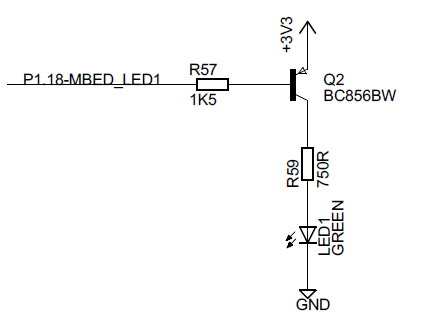
\includegraphics{led12}
  \caption{Connection for LED 1 \& 2}
  \label{fig:led12}
\end{figure}

\newthought{LED 3 \& 3 are connected to other GPIO pins.}  The circuit
is in figure \ref{fig:led34}.  The LED has current flowing through it
when the connection is high.  A logic 1 (\textsc{high}) switches on
the device.  This is why in the code, writing to the \textsc{SET}
register (setting the bit) the LED turns on.
\begin{figure}
  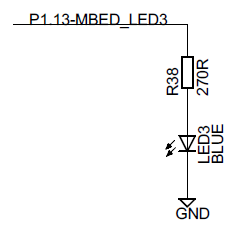
\includegraphics{led34}
  \caption{Connection for LED 3 \& 4}
  \label{fig:led34}
\end{figure}

\begin{exercise}{Extend the driver to Base-board LEDs}{extend}
From the information in the Base Board schematic \citep{baseboard},
use the information to extend the driver to the Red, Green, and Blue
LEDs.  Things to note include:
\begin{itemize}
\item What Port is the LED connected to?
\item Which Pin is the LED connected to?
\item Is the circuit active-high or active-low?
\end{itemize}
\begin{tcolorbox}[colframe=red!50!black,title=Solution]
A solution is in Git 
\begin{minted}[frame=leftline,framerule=1mm,rulecolor=\color{cmd}]{bash}
$ git checkout solution
\end{minted}
\end{tcolorbox}
\end{exercise}

\begin{question}{enum and switch}{switch}
In the code I've used a combination of \texttt{enum} for LED names,
and then a \texttt{switch} to select which code to use.  Why?
\begin{itemize}
\item What does the compiler say if the \texttt{switch} does not check
  all of the \texttt{enum} values?
\item What does the compiler warn about in the interrupt handler
  \texttt{ledone}?
\item Are these useful features?
\item How efficient is the compiled code for a switch?
\end{itemize}
\end{question}
\marginnote[-4em]{If you want to have a go at optimising the code, try
  it out.  You will find that there is a tension between compiled code
  side and ease of writing the C code.  In reality hand optimising is
  a tricky buiseness, and rarely done well.}



\bibliographystyle{plainnat}
\bibliography{lpc4088}

\appendix

\end{document}

%% Local Variables:
%% mode: reftex
%% mode: auto-fill
%% mode: flyspell
%% End:
